\chapter{State of the art} 

\chapterintro{This chapter presents recent achievements in a field of providing platform as a service by examining four vital products: Carina, OneFlow, CloudFoundry and OpenShift. It fouces mainly on aspects of adaptivity, scalability and cloud federation awareness.}

\section{Requirements}
One can notice that elements that yields a solution for a problem stated in the first chapter, which is ensuring that users' application provide appropriate Quality-of-Service for its customers in a most-cost effective manner, were gradually introduced in previous chapters:

\begin{itemize}
	\item \emph{adaptivity} - ability to adapt (i.e. scale) appropriately to a current usage pattern
	\item \emph{scalability} - ability to improve application performance by enriching resources
	\item \emph{cloud-federation awareness} - ability to compose an application deployment using different cloud providers; cooperation with different cloud provider to supply application with extra resources while performing application scaling
\end{itemize}

Next section states the general overview of the proposed solution, while the consecutive sections details its elements and finally the last section summarises the design choices in a context of system requirements.
	
% radek
\section{Carina}

\subsubsection{Overview}
Carina is an open source project, released under Apache License 2.0, built on top of OpenNebula, which aims to ``(\ldots) standardize the process for automating multi-VM deployments and setting auto-scaling and availability management policies in the cloud.'' \cite{CarinaBlog}. The project is used by the authors at their work at RIM in an OpenNebula-based private cloud.
As it is stated in the requirements of the solution, \emph{Carina} should support variety of features which can be considered worth scrutinizing carefully as they are closely related to notions of adaptivity and scalability. To name the most relevant: \cite{CarinaBlog}
\begin{itemize}
  \item Collect and aggregate OS or app-specific metrics across a cluster
  \item Drive elastic scaling of clusters based on workload or events
  \item Support deployment and handling of failover of services across multiple datacenters
\end{itemize}

Before delving into more detailed description it is vital to introduce most important terms used in \emph{Carina} documentation to depict this product:
\begin{itemize}
  \item Environment -- a collection of VMs in a master-slave configuration,
  \item Service -- a consumer of cloud resources. Each service can have its own environment configurations and create environments and control them independently of other services,
  \item Pools -- various clusters or virtual data centers in OpenNebula that can be targets for creating an environment
\end{itemize}

\subsubsection{Scaling}
Chapter 3 introduced and discussed various types of application scaling. \emph{Carina} offers only one type of scaling and this is \emph{horizontal} scaling -- user's capabilities are limited only to add/remove a virtual machine to/from a given environment. Unfortunately there are no means to modify the parameters of a given or a set of virtual machines.

In this paper we strongly advocate spanning cloud resources across multiple vendors/providers. Despite having in its requirements such a position, \emph{Carina} \textbf{does not} support deployment or scaling of services across different providers. In the environment configuration we define only \textbf{one} endpoint -- this is can be thought of a reference to a cloud provider. As it can be only one per environment, it is not possible to deploy or scale some artifacts across many providers.
\subsubsection{Adaptivity}
In \emph{Carina} there are mechanisms which can perform application scaling, both in manual and automatic fashion. It is possible for a system administrator to directly modify the existing application and its environment by changing its parameters manually. Automatic management of an environment is done by defining \emph{scaling policies} which can be in two flavours: \emph{time-based} and \emph{load-based}. Those are called by the authors \emph{elasticy policies}.

\emph{Time-based} policies defines how the system should react in the given window frame(s). In each frame we can specify the minimum number of virtual machines that comprises an environment. On the other hand, \emph{load-based} policies define the way the system reacts to \textbf{average cpu usage} by the environment. This is the simplest \emph{threshold-model} as introduced in chapter 2. The user enters predicates which are evaluated against data gathered by OpenNebula and execute scaling actions  (\emph{scaleup} and \emph{scaledown}) if they are true. What is more, the minimal and maximal number of virtual machines must be specified. At present the only parameter that is taken into account while performing actions triggered by \emph{load-based} policies is cpu usage.

To increase the application availability, \emph{Carina} introduces the notion of \emph{availability policies}. Their main function is to take a recovery action in response to a deletion or errors during deployment of a virtual machine. Recreation of a virtual machine is the most fundamental and atomic operation under this model.

\subsubsection{Design}
To complete the discussion about \emph{Carina} it is essential to include its architecture overview. This is shown in figure \ref{sota:carina-design}.

\begin{figure}[!ht]
  \begin{center}
    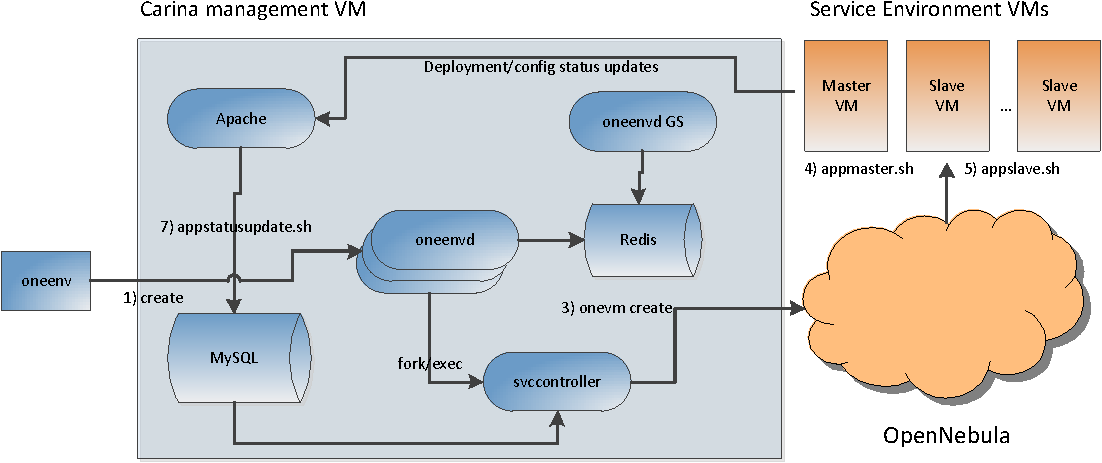
\includegraphics[width=\textwidth]{chapter-state-of-the-art/carina-design}
  \end{center}
  \caption{Carina -- components interaction}
  \label{sota:carina-design}
\end{figure}

There are number of things that cause concern:
\begin{asparaenum}
\item[\textbf{Persistency}] No one knows for what reason, but \emph{Carina} uses two databases. What makes things even worse, they completely differ in types, as \emph{MySQL} is a relational and \emph{redis} is a nosql database. This places additional burden on technical requirements of the platform.
\item[\textbf{Usage of Apache}] To work properly, \emph{Carina} needs Apache http server. In the server cgi-bin directory there are placed bash scripts which are invoked by contextualization scripts executed in different stages of virtual machines life cycle. Instead, we recommend setting proper web services, environment-agnostic, in a central node which can be run next to global scheduler.
\item[\textbf{User accounts}] \emph{Carina} forces the creation of a system-wide user for each service. These concepts should be totally independent.
\item[\textbf{Provisioning}] User has to use in the environment specification previously defined OpenNebula images. Their further adjusting happens in the contextualization phase. This forces the user to modify the state of a virtual machine when there is a need to perform any changes, for example in the software stack. Instead we suggest using some provisioning software such as puppet or chef -- this would enable users to change software stack only in configuration files (recipes) not by altering the virtual machine state.
\end{asparaenum}

\subsubsection{Summary}
\emph{Carina} emerged as a promising platform built on top of OpenNebula, which lacked most of its functionalities at that time. The good point is the fact that this product is used in a business context and judging by the authors' description it actually works. However, due to deficiencies mentioned in the previous sections, \emph{Carina} cannot be considered a mature and generic solution for more demanding cloud providers.


\section{OneFlow}

\section{OpenShift}
The section aims to answer the question: \emph{Why OpenShift is good, if at all, at what it does?} Following sections give insight into \emph{OpenShift} \cite{OpenShift} features and technical concepts, especially covering: multi-tenacy, auto-scaling and platform deployment.

\subsection{Introduction}
\emph{OpenShift} is a developed by \emph{RedHat} Platform-as-a-Service for applications. It is available in two different flavours:
\begin{itemize}
 \item OpenShift Enterprise, (private cloud)
 \item OpenShift Online / FreeShift, hosted by RedHat (public cloud)
\end{itemize}

The latter is freely available, but it is limited to only 3 gears (a 'gear' is a resource maintained by \emph{OpenShift}, such as a application server or database). Beside this, source code of this platform is hosted on github as a \emph{OpenShift Origin}, licensed with \emph{Apache License 2.0}.

\subsection{Features}
Key, high level features that distinguishes \emph{OpenShift} are:
\begin{itemize}
  \item \emph{Accelerated Application Service Delivery} by on-demand and self-provision application stack access
  \item \emph{Minimised Vendor Lock-in} by portability (there is no proprietary APIs, technologies)
  \item \emph{Automatic Application Scaling}
\end{itemize}

Beside this, main features include:
\begin{itemize}
  \item \emph{Polyglot} - there is a number of built in application stacks (jee, ruby, python, databases); user is allowed to defined one himself through a concept of 'cartridge'
  \item \emph{One Click Deploy} - application are managed by OpenShift through git repository. Deploying new version of application comes down to pushing new version application's source code.
  \item \emph{SELinux-based Secure Containers for multi-tenancy}
  \item \emph{Automatic Application Stack Provisioning}, it is only necessary to specify required cartridge (application stack) and all the dependencies are provided by platform
\end{itemize}

\subsection{Key technical concepts}

\subsubsection{Multi-tenancy}
In \emph{OpenShift}, each application is represented as a set of gears. For example, gear is a database or application server. Such gears are hosted on \emph{OpenShift Nodes}. There is a many-to-one relationship between gear and \emph{OpenShift Nodes}. What is leveraged to achieve this multi-tenancy is:
\begin{itemize}
 \item SELinux, isolation between application running at the same node
 \item Control Groups (cgroups), fine-grained control over the memory / CPU / IO utlization / networking on per process basis
 \item Kernel namespaces, groups of processes are separated, so that they cannot see resources in other groups
\end{itemize}

\subsubsection{Auto-scaling}
While creating new application, it is possible to specify whether application should scale (later this setting cannot be changed). Provided that scaling is enabled, additional gear is allocated to host \emph{HAProxy} \cite{HAProxy}.

In order to scale, \emph{OpenShift} uses a relatively straightforward algorithm \cite{OpenShiftScaling}:
\emph{
\begin{quote}
The algorithm for scaling up and scaling down is based on the number of concurrent requests to your application. OpenShift allocates 10 connections per gear - if HAProxy sees that you're sustaining 90% of your peak capacity, it adds another gear. If your demand falls to 50% of your peak capacity for several minutes, HAProxy removes that gear.
\end{quote}}

\subsubsection{Cloud federation}
Before getting into discussion about possible work in a cloud federation environment, it is necessary to recap \emph{OpenShift's} deployment process.

\begin{asparaenum}
  \item[\textbf{Deployment}] As one may notice in 'Multi-tenancy' section, \emph{OpenShift} does not provision application as virtual machines. Instead they are simply processes running on \emph{OpenShift Nodes}, which themselves are instances of \emph{RedHat Enterprise Linux}. The \emph{OpenShift Enterprise (private cloud )} is a flavour that allows for choosing underlying infrastructure running \emph{RHEL}. It can be a physical node as well as virtual machine, managed, for example, by OpenStack. 

  \item[\textbf{Hybrid configuration}] As previous point highlights, \emph{OpenShift} doesn't use any notion of a datacenter / service provider. Consequently, it not possible to \emph{OpenShift} to cooperate in an intra-datacenter / service provider environment.
\end{asparaenum}

\subsection{Summary}
Summing up, key advantage of the \emph{OpenShift} seems to be it simplicity: creating and deploying applications using \emph{OpenShift} is as simple as it gets. Beside this, built in support for most popular technologies and simple API for OpenShift attractive platform. Having that said, auto-scaling and being constraint to a single cloud provider may be not sufficient in complex scenarios.

% radek
\section{CloudFoundry}


% radek
\section{Providers comparison}
	
